\section{Method and Data} 
\label{sec:method}
From a holistic view of research method (Figure~\ref{fig:System structure}), it
consists several relational parts of the dataset import,dataset Processing, and machine model training for topic clustering

In dataset import process, since the dataset is un-hydrated, we needed
to “hydrate” the data by building a process that will fetch the tweet content
by querying with the Tweet ID. After hydrating, the data are saved in a local
storage, and by using Tweets API the data are completed to be analyzed and
stored in the Elasticsearch server. 
\begin{figure}[h]
\centering
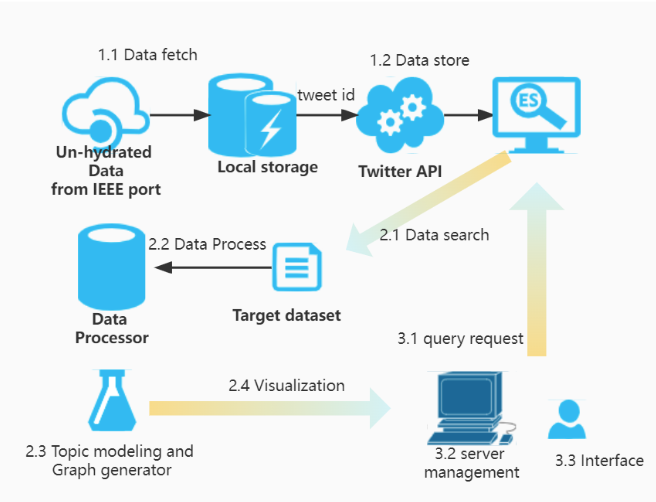
\includegraphics[width=0.5\textwidth]{imgs/framework/framework.png}
\caption{System structure}
\label{fig:System structure}
\end{figure}
In dataset processing step, after importing data into Elasticsearch server in
batches, we choose a research scope and we get the target dataset from
Elasticsearch. By doing spatial query and filtering task, the target dataset
can be visualized into a map. Furthermore, after processing the data by using
techniques such as the regex filtering, tokenization and tagging, and
removing stop words, it is possible to apply a topic clustering model to get topics.





\subsection{Sentence vector generation}
We propose to use a LDA-BERT based method to generate vector for each tweet. First, we break down tweets into body and hashtags. For the body part, we tokenize the sentences and train them with BERT. Then we get vectors which contains hundreds of dimensions. For the hashtags part, we apply LDA on them and generate vectors of corresponding dimensions according to the number of topics to be divided into. To combine the information form two resource, we use autoencoder to compress combined vector.

\begin{figure}[h]
\centering
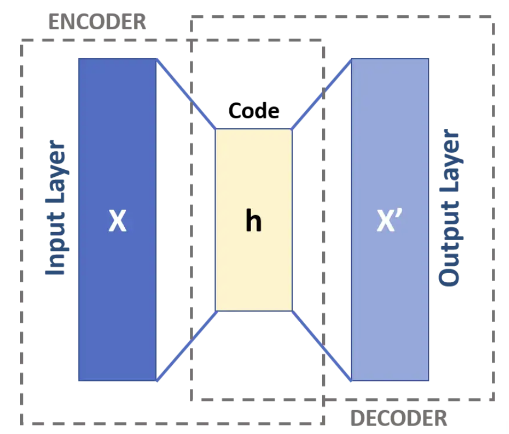
\includegraphics[width=0.5\textwidth]{imgs/framework/autoencoder.png}
\caption{structure of autoencoder}
\label{fig:autoencoder}
\end{figure}

By this method, we succeed in reducing the dimensionality of the resulting vector while preserving topic features.

\subsection{Topic Clustering}
We use Time Series KMeans to do the clustering. Because each tweet is attached with publish time, we need to consider its temporal correlation while clustering. 

\subsection{Visualization}
\subsubsection{Wordcloud}
Wordcloud is a graph to show the high frequency words. After clustering, we get labels which indicate which cluster the current tweet belongs to. Then we get all word lists under the same cluster and concat them. Finially the wordcloud will show higher frequency words in bigger font.
\subsubsection{Centroid sentence}
To study topic relevance, we calculate the cosine similarity between every tweet and cluster centroid point and pick up the nearest tweet as the most representative tweet.  
\subsubsection{Storyline}
To generate a graph showing all topic relationships, we caculate the similarity between all the topic pair. Then sort the calculation results from high to low. Based on it, we set a threshold of edge. An edge will be generated between all topic pairs whose similarity is greater than the threshold. Finally we import the point and edge information into Graphviz and get a graph.(Fig~\ref{fig:storyline for lda_bert}) 
